
\chapter{Method (HOW)}
\label{chp:method}
\section{On the content}
Here you specify and motivate your research questions or hypotheses and relate them to your overall goal, research question, or hypothesis, if you have defined one in the introduction. Furthermore, you describe the method or research design for answering your research questions or testing your hypotheses and discuss the reliability and validity of your approach. The latter is important for a reader to assess the trustworthiness and generalizability of your results.  


\section{Defining research questions}

\section{Preliminary goals:}
\normalsize
\begin{enumerate}[label=PG\arabic*., leftmargin=*]
    \item Create a proof of concept of a highlight algorithm, that finds "better" highlights for a given player in a match
    \item Find out what is required for an alternative highlight algorithm, what metrics players prefer
    \item Find what makes a highlight "better" and increases enjoyment when watching a highlight.
\end{enumerate}

\section{Preliminary research questions:}
\normalsize
\begin{enumerate}[label=RQ\arabic*., leftmargin=*]
    \item How can one create an algorithm to find better highlights in Counter Strike 2? \\\\
    The value of creating the proof of concept is a better highlighting algorithm than existing ones, thus making for better clips for players and spectators of the game. 
    \item What metrics are most important when developing an algorithm to find highlights in Counter-Strike 2? \\\\
    Finding out what is required for a highlight and what players prefer can help in further research into the subject and can even connect to other games where similar highlights can be of interest.
    \item How do the perceptions of what makes a good highlight differ between novice and experienced players?\\\\
    Finding out the difference between perception of highlights of a seasoned player or someone who has not as much or no experience gives us a insight how you can direct highlights so that they can be enjoyed by different demographics. 
    
\end{enumerate}
Research question number 1 is connected to goal 1. Question 2 is connected to goal 2. Question 3 is connected to goal 3.\\\\
The value of these goals can affect and be used by players of the Counter Strike 2, others that are interested in the topic of highlight making/analyzing, and for spectators of the game.\\\\

\section{Describing your research method}
We use a proof of concept and mixed-methods approach with surveys and interviews in this study. The interviews are conducted to get a better insight into what and how to weigh different metrics that will be used in the algorithm. The surveys serve the purpose of comparing our algorithm with existing highlight tools. This way we can see if our algorithm could be considered better at finding highlights.
\subsection{Proof of concept of an algorithm}

\subsubsection{Initial plan}
The initial plan was to have a system in which the \Gls{Demofile} is analyzed and all the results of the different metrics are multiplied by a weight and then added to a final score. Some of the metrics are ones that you want to be lower, like the time between each kill, and if you die. The formula would look something like this.

$$\text{Total Score} = \sum_{i=0}^{x} weight_i \times metric_i $$

where x is the number of metrics

\subsubsection{Implementation}

Implementing the analyzer step was a lot of code to write, but not much advanced code. Mostly it was reading some value for each player every round, and storing those values in a Metrics class. This class held all information about a players metric for a given round, and contained some helper methods to set the metrics in a cleaner way.

One of the metrics that was hard to implement was the \Gls{jumpshot}s. Until very recently (2024-04-24), there was no built in way of checking if a player was in the air or not, but right in time, Valve, the developer of Counter strike 2, added a new feature\cite{onTheOtherHandReleaseNotes} to show if a player is in the air during a kill.

Before this, our solution was to check the Y position of the player over a two second windows, one second before until one second after. After this, we checked the position of the player and made sure that the players velocity was an arch, starting going high, and then curving back down. This solution has issues, a ladder or stairs could fool this solution, so the newer update was very helpful.

\subsubsection{Final Product}

The final product contains a web interface, that made it easier for us to use and look at the metrics and whats going on. This was helpful for debugging issues with the analyzer, as well to see why a round got the score it did. The full process is that you upload the demo file you want to analyze onto the site, this gets passed to a DemoAnalyzer instance, that extracts the demo information. This then loads up a page where we can see all the metrics, for all the players, in all rounds. The round score for each round is automatically calculated, and the best round score of the match gets displayed on the site, along with the metrics for that round. This is how we determined what clips were supposed to be used for the survey. The web page could be adapted for user consumption, by just hiding the details of the round.

\paragraph{Linear Metrics}
For all linear metrics that we have, we map the input to somewhere between 0 - 100. This was we handle cases where two metrics are of the same importance, but the value they give are orders of magnitude off each other. An example would be damage, and kills (genom) smokes. You can only get a maximum of 5 kills trough smokes, but you can get up to 500 damage. This was if i get 2 smoke kills and 200 damage, both will output 40. We used a linear mapping function for this. The function is explained below

The metrics that use this method of scoring is:
\begin{itemize}
    \item Damage dealt
    \item Head shots
    \item No-Scopes
    \item How long between each kill
    \item \Gls{jumpshot}s
    \item Hit ratio
    \item Distance
\end{itemize}

\begin{align*}
& \textbf{Function map:} \\
& \text{map}(v, v_{\text{min}}, v_{\text{max}}, t_{\text{min}}, t_{\text{max}}) = \frac{v - v_{\text{min}}}{v_{\text{max}} - v_{\text{min}}} \cdot (t_{\text{max}} - t_{\text{min}}) + t_{\text{min}} \\
& \quad \text{where:}\\
& \quad \quad v: \text{input value}\\
& \quad \quad v_{\text{min}}: \text{minimum input value}\\
& \quad \quad v_{\text{max}}: \text{maximum input value}\\
& \quad \quad t_{\text{min}}: \text{minimum target value}\\
& \quad \quad t_{\text{max}}: \text{maximum target value}\\ \\
& \textbf{Function mapToScore:} \\
& \text{mapToScore}(v, v_{\text{min}}, v_{\text{max}}) = \text{map}(v, v_{\text{min}}, v_{\text{max}}, 0, P) \\
& \quad \text{where:}\\
& \quad \quad P:  \text{represents the constant POINTS\_PER\_METRIC = 100}
\end{align*}

This function is the same used by a popular library p5js \cite{p5jsMap}, that is used for interactive graphics among other things. We made a shorthand to write cleaner code, using the function mapToScore, that calls the map function, but with the target min and max values already set to 0 and POINTS\_PER\_METRIC, that in out case is 100


\paragraph{Exponential metric}
For some metrics, we choose to make a greater difference between the lower numbers and the higher ones. We did this by raising the input to the power of 2 before using the mapToScore function. This was we get a bigger difference between 4 and 5, compared to 2,3. This we only did for kills.

\paragraph{Other metrics}
Some metrics did not work well with this system, since they either are not numbers, or needed other processing on them to make them work well inside the algorithm. This section will explain how they work, and why they did not work with the linear or exponential functions. Some of them just mapped to either the maximum amount of points, like if you died, or what side you were on.
\paragraph{HP left}

This uses a exponential decay function. This is because the lower the health of the player, the more stress it puts on the player. \todo{reference to interviews, and write more about why we choose 35}. We picked 35 as the point where we should start increasing the points significantly. We can now input the \acrshort{hp} of the player into the formula and we get a value between 5 and 100.            
$$x) = 100 \cdot e^{-ax}  \qquad \text{where } a = 0.03$$
This is then mapped using the function mapToScore from before to a number between 0 and 100. After the normalizing we multiply this by the weight for the metric. 
\todo{explain how the function works and how we came p with it}
This formula is an exponential decay function. It models the decrease in \acrshort{hp} Left Value as the input value (x) increases. The growth rate (a) controls how quickly the value decays. A higher growth rate means a faster decay. \todo{CHATGPT WRITTEN}

We choose 0.03 as the $a$ value since this makes the points for that metric go up around the 35 \acrshort{hp} mark, that being one shot away from death from most strong weapons.


\begin{figure}
    \centering
    \begin{tikzpicture}
\begin{axis}[
    axis lines = left,
    xlabel = $HP$,
    ylabel = {$f(x)$},
]
\addplot [
    domain=0:100, 
    samples=100, 
    color=blue,
] {100 * exp(-0.03*x)};
\addplot[
    only marks,
    mark=*,
    nodes near coords,
    point meta=explicit symbolic,
]
coordinates {
    (35, 100 * exp(-0.03*35)) [One Shot]
};
\end{axis}
\end{tikzpicture}
    \caption{HP left scaling}
    \label{fig:hp-left}
\end{figure}

\paragraph{Weapon score}
For the weapons, we decided to score each weapon individually, this was each weapon gets a part of the max score for the metric. This is done by first dividing the total score for the metric, so for four weapons that will be 25 points. Then it used that value as the max points for the weapon, and rates it with the difficulty rating from the game, taken from the ingame buy menu. For an ak47, which has a difficulty rating of 4, the formula is as follows: $$ score = map(weaponDifficulty, 0, MWW, 0, PPW) $$ Here MWW is max weapon weight, and PPW is points per weapon.

This is done for each one of the weapons added together and finally multiplied with the weight for guns.


\paragraph{Side}
When looking at what side the player is playing on, either \acrshort{t} or \acrshort{ct}, we looked at the win rate for each side for the last 6 months\cite{hltvMapStats}. Here we saw a quite even split, but based on the map in the current competitive map pool, \acrshort{ct} has a higher win rate on the majority of the maps. Therefore we assign \acrshort{t} and \acrshort{ct} -1 and 1, then in the weights, it has a negative value, so that the -1 for \acrshort{t} get awarded more points than \acrshort{ct}.


\subsubsection{Technologies used}
Our algorithm was built using Typescript as the language of choice. This choice was made both out of familiarity and based on Typescripts fast iteration speed, enabling us to make changes faster than a language like C++ or Rust.

Counter-strike 2 records everything that happens in a match in a \Gls{demo} file. To parse this information, we used a library\cite{demoparser} that would give us events from the match, such as whenever a player dies, shoots, or when the rounds start or end. This library does not give us the data we need directly, so for that we need to parse information from the events available. So for that we need to analyze the data from the demo, to later pass to our algorithm to calculate with \todo{EXPLAIN MORE????}
\subsubsection{How it works}
The first part of the process to generate a highlight is to extract the metrics from the demo file. This is done in a file called DemoAnalyzer.ts, and this fine handles reading the \Gls{demo} file and transforming the data into a usable format. It does this by looking at different events \todo{list events??} and calculate the metrics. \todo{explain how some of them work?}.

The next part is to store the metrics in the database. This is handled by a separate file `SaveDemoInfo.ts`. This file reads the data, and puts it into tables in the database. The reason for making this a separate step was for readability and code quality. This splits up the code into the analyzer, that is only responsible for reading the data, and storing it in memory, and the SaveDemoInfo part, that only focuses on storing the data. 

The last part is the most important step. This is the algorithm itself. This takes in all the data from the demo file, as well as the weights we have defined from the interviews \ref{sec:interviews}. This then calculates a score from each metric between 0 and 100. This was done to make sure that each metric is valued the same before the weighing process. This is done using this mapping function from p5.js\cite{p5jsMap}\todo{check ref with henry}

After the mapping function has given its value between 0 and 100, this then is weighted, so that we can control how important the metrics are for a highlight. For example, should one kill through a wall be considered better or worse than one kill that is very far away? That is the proposal of a weight. \todo{better example?}

\subsection{Survey}
\label{sec:survey}
A survey will be created with our algorithm's outputted round and the Allstar{glossarie} tool's "play of the game" round, where the same matches are evaluated on the same player, and the participant can choose which they prefer. Both rounds will be re-recorded so that a fair comparison can be made without editing and each clip starts a few seconds before and action such as shooting, spotting an enemy or throwing utility is done.\\\\
\textbf {Content for the survey:}
\begin{itemize}
    \item The respondent will be prompted to answer a question about how familiar they are with the game Counter-Strike 2. This will be presented in a type of likert scale. 
    \begin{figure}[H]
        \centering
        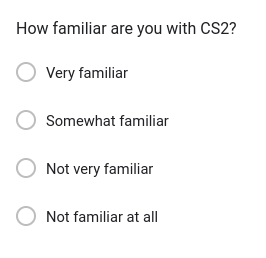
\includegraphics[width=4cm]{Images/likertscale.png}
        \caption{Likert scale}
        \label{fig:likerScale}
    \end{figure}
    \item Two clips are shown, A and B. One is the round our algorithm picked and one is the round Allstar picked, the respondent will not be told which clip is which so that there will be no biases. The respondent is then faced with the question of which clip they preferred or if the clips are indifferent. They then have the choice to write a more detailed explanation why they picked as they did or any other input they had. There will be 18 clips in total, 9 comparisons.
    \begin{figure}[H]
        \centering
        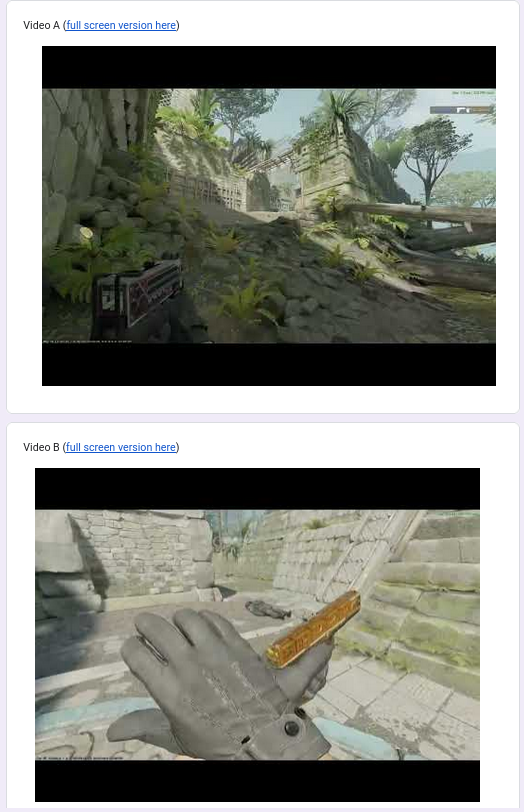
\includegraphics[width=10cm]{Images/A-B_choices.png}
        \caption{Video A and B example}
        \label{fig:VideoA_B}
    \end{figure}
    \begin{figure}[H]
        \centering
        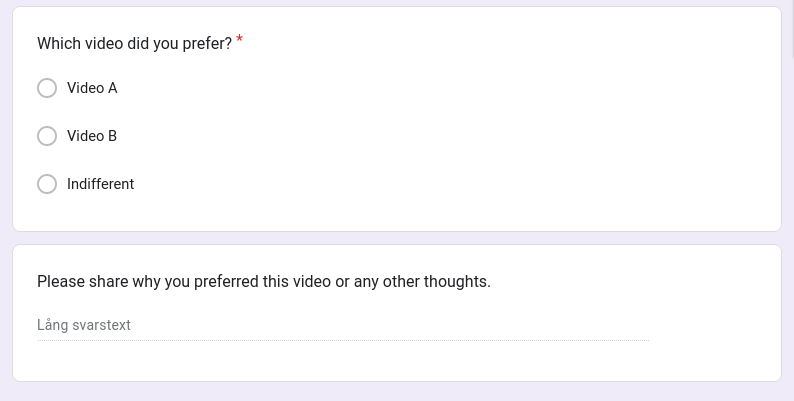
\includegraphics[width=10cm]{Images/Questions_AB_reason_Survey.png}
        \caption{Video A and B example}
        \label{fig:VideoA_B_answer_reason}
    \end{figure}

\end{itemize}
The survey will connect with preliminary goal 1 to see if our the highlight our algorithm creates are preferred over what existing tools create. It will also answer research question 3 by seeing if algorithm based highlight clips can create joy for the viewer.\\\\
The choice to conduct surveys was made because we want to have a large pool of opinions, as we want to see if our new algorithm is "better" than existing ones. By choosing to do surveys, we can reach a greater amount of people. To create the surveys, we would use either sites like Surveymonkey.com or Google Forms. The surveys would be put in different forums on sites like Reddit.com, Discord channels and HLTV.org. The main targeted respondents would be those who have played Counter Strike 2, as these are the more likely to have an opinion about the clips they are shown. As we have no control of the surveys and who receives them, we would likely need to put questions such as "Have you played the game Counter Strike 2?" to see the difference in opinions between people who have played the game and not.\\\\
When analyzing the results, we would need to do a statistical analysis of the quantitative data, which would be the preferred clip. We could then gather statics such as the median for which clips the users decide to pick. Creating pie charts would also be a good way to visualize how the participants picked. For the qualitative data, which would be the free text part where the participant explained why they picked what, we will have to look for patterns and trends between what they picked and categorize based on if they played the game before.

\subsection{Interviews}
\label{sec:interviews}
Interviews will be conducted before developing the algorithm to find what metrics players weigh higher, to give a better baseline on what the weights should be. \\ \\
\textbf {Questions for the pre interview:}\\
\section{Questions:}
\normalsize
\begin{itemize}
    \item What is the most memorable highlight in Counter Strike history according to you? 
    \begin{itemize}
        \item What makes it memorable?
    \end{itemize}
    \item What is your experience with highlights in FPS games?
    \item What makes a good highlight?
    \item What metrics are important for a highlight?
    \item Rate these metrics from 1 to 10:
        \begin{itemize}
        \item Amount of kills 
        \item if the player died
        \item Weapon used 
        \item Time between each kill
        \item Bullets fired
        \item Team side
        \item Player position (Distance)
        \item Airborne 
        \item Headshot
        \item Damage given
        \item HP of the player
        \item No scope with scoped weapons
        \item Wall banging
    \end{itemize}
    \item Do you use any highlight tool?
    \begin{itemize}
        \item What highlight tool?
        \item What do you do with the highlights?
    \end{itemize}

    
\end{itemize}

Question one to three in the pre interview will help us achieve the three preliminary goals and answer the research questions, as these will give us further insight into what metrics are needed and how to value them. It will also help us get a better insight to what makes a good highlight. \\\\
The choice of doing interviews was so that we could get a better understanding on how to rate different metrics and what players think is a good highlight so that we could improve our algorithm. The interview would be conducted either in person or online, where it would be recorded or transcribed. The targeted respondents would be people who analyze the game, such as casters, commentators or professionals players of the game. We would also interview more casual players of the game. To recruit these respondents, we would have to email or contact them through other forms and ask if they are interested in participating in our interview. After the interviews are conducted, we gather all the data we have collected and analyze it. Things to look for would be patterns and themes that are recurring in the answers.\\\\
The answers we gathered here lays a base on how we weigh our metrics but could be used in other games that are similar to Counter Strike 2.\\\\ 

\section{Validity and reliability of your approach}
Our approaches of collecting data through interviews was done via discord where we recorded the interview. This was done so that we could have a greater reach of who we interviewed. This made it possible to get a bigger size pool of different people. We also had to take into account that the people we wanted to interview had played Counter Strike or similar games.\\\\ We recognized that it would be hard to fairly value metrics, as there a many, but the approach we took made it so that if there are metrics not mentioned by us in the interview the interviewee could have the possibility to add metrics.\\\\
Our approaches of collecting data through surveys was done via Google forms to compare our algorithm with the existing highlight tool ALLSTAR. The participants would not know which clip came from ALLSTAR or our algorithm. As the clips created are from the same matches and the same persons when comparing this makes it as un-biased as possible. The games where from our own games history from the dates {INSERT DATE} to {INSERT DATE}. In case our algorithm and Allstar outputted the same round a new match was picked and the instance noted down. 